\documentclass[10pt,serif]{beamer}
\usepackage{latexsym}
\usepackage{amsmath}
%\usepackage{mathspec}
\usepackage{amsthm}
\usepackage{amssymb}
% \usepackage{textcomp} 
% \usepackage{ulem}
% \usepackage{fontspec}     
\usepackage[british]{babel}
\usepackage{enumitem}
% \usepackage{pifont}
\usepackage{geometry}
\usepackage{hyperref}
\usepackage[table]{xcolor}
\usepackage{tikz}
\usepackage{colortbl}
% \usepackage{mathrsfs}

% \usepackage{eucal}
\usepackage{dsfont}
% \usepackage[most]{tcolorbox}
% \usepackage{mathdots}
\usepackage{minted} %? used for code-integration
% \usepackage{titling}
\usepackage[citestyle=alphabetic,bibstyle=alphabetic]{biblatex}
\definecolor{darkmagenta}{rgb}{.38,0,0.38}
\hypersetup{
    colorlinks,
    citecolor=darkmagenta,
    filecolor=darkmagenta,
    linkcolor=darkmagenta,
    urlcolor=darkmagenta
} %? Change hyperlink's styles

%%%%%%%%%%%%%%? courbes
\usepackage{amsfonts,amscd}
\usepackage{pgfplots}
%%%%%%%%%%%%%?

%%%%%%%%%%%%%
\DeclareMathOperator{\mat}{Mat}
\DeclareMathOperator{\card}{Card}
\DeclareMathOperator{\len}{len}
\DeclareMathOperator{\erf}{erf}
%%%%%%%%%%%%%


%%%%%%%%%%%%%
\newcommand{\dt}{\mathrm{d}}
\newcommand{\un}{\mathds1}
\renewcommand{\o}{\scriptstyle\mathcal{O}}
\renewcommand{\O}{\mathcal{O}}
\renewcommand{\emptyset}{\varnothing}
\newcommand{\lbd}{\lambda}
\renewcommand{\phi}{\varphi}
\def\inte #1 #2 { [\![#1,#2]\!] }
%%%%%%%%%%%%%


%%%%%%%%%%%%%
\newcommand{\N}{\mathbb{N}}
\newcommand{\R}{\mathbb{R}}
\newcommand{\Z}{\mathbb{Z}}
\newcommand{\C}{\mathbb{C}}
\newcommand{\K}{\mathbb{K}}
\newcommand{\Q}{\mathbb{Q}}
\renewcommand{\P}{\mathbb{P}}
\newcommand{\M}{\mathcal{M}}
\renewcommand{\r}{\mathcal{R}}
\renewcommand{\S}{\mathcal{S}}
%%%%%%%%%%%%%


\renewcommand{\arraystretch}{1.4} %? For better matrix
\renewcommand{\thesection}{\arabic{section}} %? Roman number for sections

% \theoremstyle{definition}
% \newtheorem{definition}{Definition}[subsubsection]

% \theoremstyle{theorem}
% \newtheorem{theorem}{Th\'eor\`eme}[subsubsection]

% \theoremstyle{lemma}
% \newtheorem{lemma}[theorem]{Lemme}

% \theoremstyle{corollary}
% \newtheorem{corollary}{Corollaire}[theorem]

% \theoremstyle{remark}
% \newtheorem*{remark}{Remarque}


\newenvironment{code}{
    \VerbatimEnvironment
    \begin{minted}[mathescape,
        linenos,
        numbersep=5pt,
        gobble=2,
        frame=lines,
        framesep=2mm]{cpp}%
}{
        \end{minted}%
}


% \flushbottom




\usetheme{CambridgeUS}
\usecolortheme{rose}
\setbeamercolor{frametitle}{fg=darkmagenta}
\setbeamercolor{title}{fg=darkmagenta!80!white}

\setbeamercolor{palette primary}{fg=black, bg=gray!30!white}
\setbeamercolor{palette secondary}{fg=black, bg=gray!20!white}
\setbeamercolor{palette tertiary}{fg=white, bg=darkmagenta}
\setbeamercolor{palette quaternary}{bg=darkmagenta, fg=white}

% \setbeamersize{
%   text margin left = 0.25cm, % normalement c'est 1 cm
%   text margin right = 0.25cm % normalement c'est 1 cm
% }



%% Pour supprimer la barre de navigation
\beamertemplatenavigationsymbolsempty

% \newlength{\hauteurFrameTOC}
% \setlength{\hauteurFrameTOC}{0.65\textheight}
% \newlength{\upTOC}
% \setlength{\upTOC}{-10pt}


% \AtBeginSection[]
% {
%   \begin{frame}<beamer>
%     \frametitle{Sommaire}
%     \vspace{\upTOC}
%     \hfill
%     \parbox[t]{.95\textwidth}{
%       \begin{minipage}[c][\hauteurFrameTOC]{\textwidth}
%         \tableofcontents[currentsection]
%       \end{minipage}
%     }
%   \end{frame}
% }


% Pour changer le stye des points itemize
% \setbeamertemplate{itemize item}[triangle]

% \newlength{\lengthleft}
% \newlength{\lengthright}


% \setbeamertemplate{headline}[default]
% \setbeamertemplate{footline}[default]

% \defbeamertemplate*{footline}{infolines theme}
% {
%   \hbox{%
%     \begin{beamercolorbox}[wd=.22\paperwidth,ht=2.25ex,dp=1ex,center]{author in head/foot}%
%       TIPE 2021
%     \end{beamercolorbox}%
%     \begin{beamercolorbox}[wd=.70\paperwidth,ht=2.25ex,dp=1ex,center]{title in head/foot}%
%       \insertshorttitle
%     \end{beamercolorbox}%
%     \begin{beamercolorbox}[wd=.08\paperwidth,ht=2.25ex,dp=1ex,center]{author in head/foot}%
%       \insertframenumber/\inserttotalframenumber
%   \end{beamercolorbox}  }%
% }

% Supprime les ombres des block (ces trucs buguent aujourd'hui)
\setbeamertemplate{blocks}[rounded][shadow=false]


% Pour cacher des frames:
% \newcounter{FrameNumberBeforeAppendix}
% \newenvironment{annexes}{
%   \setcounter{FrameNumberBeforeAppendix}{\value{framenumber}}
% }{
%   \setcounter{framenumber}{\value{FrameNumberBeforeAppendix}}
%%}


\usepackage{subcaption}

\def\bibfont{\footnotesize}
% \renewcommand\bibliographytypesize{\small}
{\footnotesize
\bibliography{../Report/main.bib}}
\usepackage{wrapfig}
\usepackage{ragged2e}
\usepackage{tabularx}
\usepackage{tkz-base}
\usepackage{tikz}
\usepackage{csquotes}
\usepackage{pgfplots}
\usepackage{datetime2}
\usepackage{adjustbox}
\usepackage{cleveref}
\usepackage{multicol}
\usepackage{graphicx}
\usepackage{multirow}
\usepackage{tabularx}
\usepackage{multimedia}



\newcolumntype{C}{>{\centering\arraybackslash}X}
\newcolumntype{s}{>{\hsize=.3\hsize\linewidth=\hsize}C}
\newcolumntype{D}{>{\hsize=.4\hsize\linewidth=\hsize}C} %Double width column


\AtBeginSection[]
{
  \begin{frame}
    \frametitle{Table of content}
    \tableofcontents[currentsection]
  \end{frame}
}

\uselanguage{English}
\languagepath{English}

\pgfplotsset{compat=1.17}
\renewcommand{\today}{\number\day\textsuperscript{\scriptsize\text{th}} \DTMenglishmonthname{\month} \number\year}
% \useoutertheme{smoothbars}

% \setbeamertemplate{title page}[default][colsep=-0bp,rounded=false]
% \setbeamertemplate{frametitle}[default][colsep=-4bp,rounded=false,shadow=false]
% \setbeamertemplate{blocks}[rounded][shadow=false]
% \setbeamertemplate{headline}[shadow=false]
% \setbeamertemplate{subsection in head}[shadow=false]
% \setbeamertemplate{section in head}[shadow=false]
% \setbeamertemplate{beamercolorbox}[shadow=false]

\makeatletter
\def\@makefnmark{}
\makeatletter

% \setbeamertemplate{footnote}{%
%   \parindent 1em\noindent
%   \raggedright
%   \insertfootnotetext\par
% }

%%%%%%%%%%%%%%%%%%%%%%%%%%%%%%%%%%%%%%%%%%%%%%%%

% \title{
%   Arbitrages statistiques dans l'apprentissage automatique confidentiel
% }
% \author{{\sc Alexi Canesse}\\ Candidat 557}
% \date{\today}

\title[] %optional
{EEG and MEG Data Preprocessing}

\subtitle{Oral presentation}

\author[Esteban Christiann, Alexi Canesse]{{Alexi \sc Canesse} and {Esteban \sc Christiann},\\ ENS Paris-Saclay, France}

\institute[] % (optional)
{
    Project for the time series course\\
    Part of the MVA program at ENS Paris-Saclay.\\
}

\date[Oral presentation] % (optional)
{\today}

% \logo{\includegraphics[height=1cm]{}}

%%%%%%%%%%%%%%%%%%%%%%%%%%%%%%%%%%%%%%%%%%%%%%%%

% \pgfplotsset{every axis/.append style={
%         scaled y ticks = false,
%         scaled x ticks = false,
%         y tick label style={/pgf/number format/.cd, fixed,
%                             int detect,1000 sep={\;},precision=3},
%         x tick label style={/pgf/number format/.cd, fixed, fixed zerofill,
%                             int detect, 1000 sep={},precision=3}
%     }
% }

\setlength{\parskip}{1em}

\begin{document}
% \addbibresource{pres.bib}


\begin{frame}
  \titlepage
\end{frame}

\section[\color{white} Introduction]{Introduction}\label{sec:introduction}

\begin{frame}{Introduction}

  EEG and MEG data are prone to a lot of different artefacts such as steps, ringing, slow drift and glitches.

  The article we studied introduces methods to preprocess EEG and MEG data.

  \begin{figure}
    \centering
    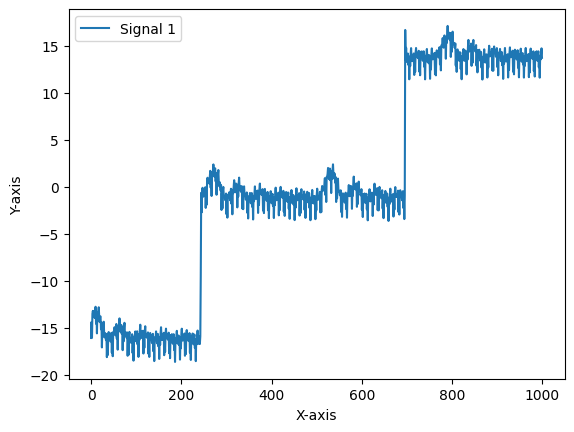
\includegraphics[width=.3\textwidth]{figures/steps_exemple}
    \hfill
    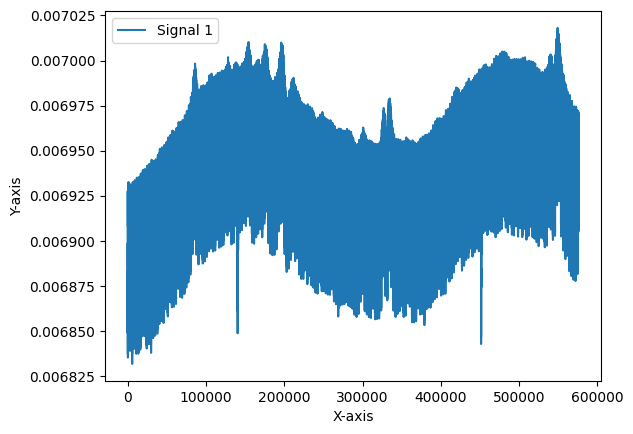
\includegraphics[width=.3\textwidth]{figures/trend_exemple}
    \hfill
    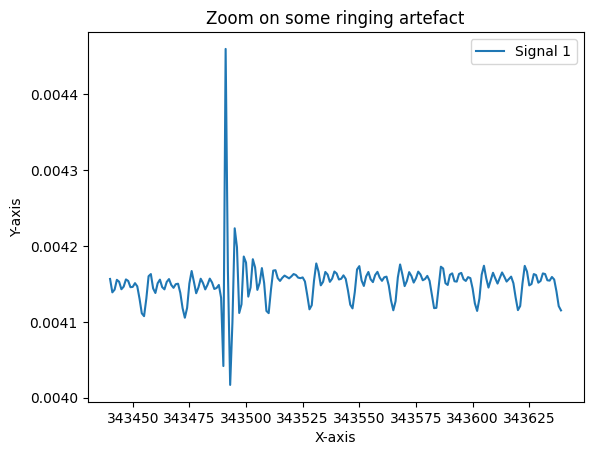
\includegraphics[width=.3\textwidth]{figures/ringing_exemple.png}
    \caption{MEG steps on the left, trend on the middle and ringing on the right.}
\end{figure}

\end{frame}

\begin{frame}{Contributions}

\end{frame}

\section[\color{white} Methods]{Methods}\label{sec:methods}

\begin{frame}{Robust detrending}
    Usual detrending methods are sensible to artefacts.

    $\implies$ Robust detrending: estimate the trend ignoring outliers, and flag high errors as outliers for the next iteration
    \begin{figure}
        \centering
        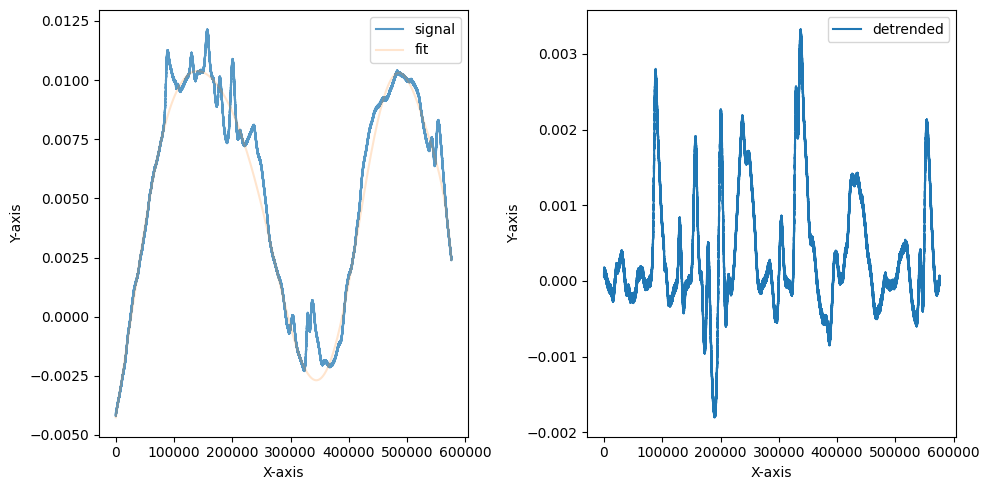
\includegraphics[width=.8\textwidth]{figures/detrend_real.png}
        \caption{Application of the detrending algorithm.}
        \label{fig:data}
    \end{figure}
\end{frame}

\begin{frame}{Inpainting}
    Inpainting is the process of reconstructing the signal at timesteps affected by glitches. Here, we assume that glitches locations are known.

    This algorithm first estimates the linear relationship between channels and use it to reconstruct the signal.
    \begin{figure}
        \centering
        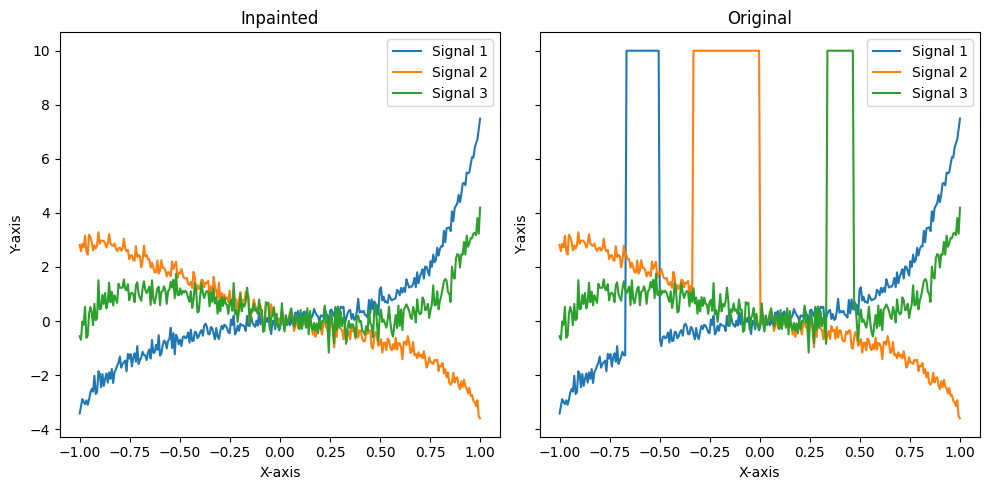
\includegraphics[width=.7\textwidth]{figures/inpaint.png}
        \caption{Application of the inpainting algorithm.}
        \label{fig:data}
    \end{figure}
\end{frame}

\begin{frame}{Outlier detection}

    To flag outliers, we use the previous algorithm and flag poorly reconstructed values as outliers for the next iteration.

    \begin{figure}
        \centering
        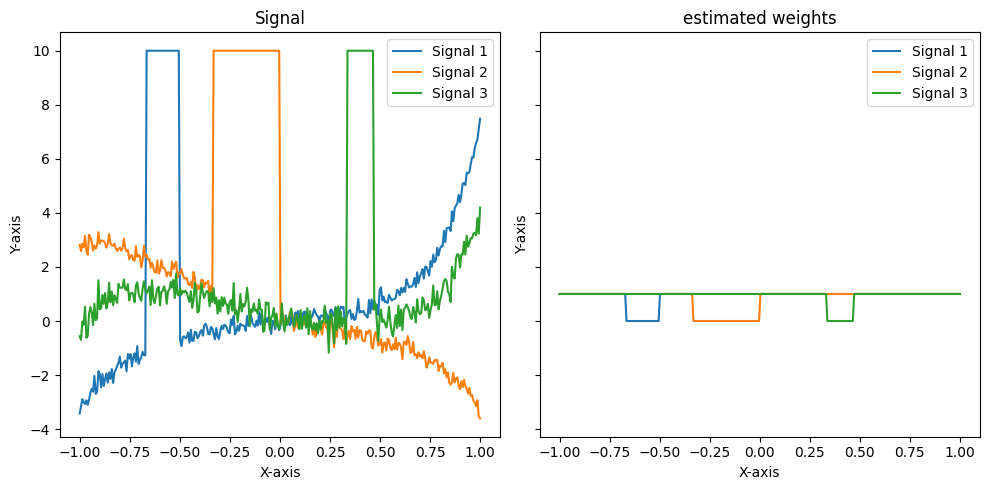
\includegraphics[width=.8\textwidth]{figures/outlier_detection.png}
        \caption{Application of the outlier detection algorithm.}
        \label{fig:data}
    \end{figure}

\end{frame}

\begin{frame}{Robust rereferencing}

    \begin{figure}
        \centering
        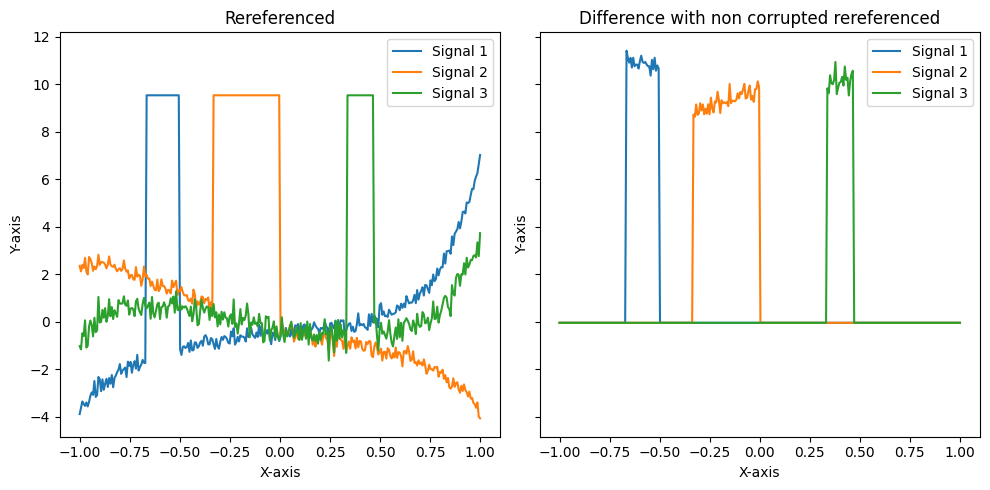
\includegraphics[width=.8\textwidth]{figures/rereferencing.png}
        \caption{Application of the robust rereferencing algorithm.}
        \label{fig:data}
    \end{figure}

\end{frame}

\begin{frame}{Step removal}
    \begin{figure}
        \centering
        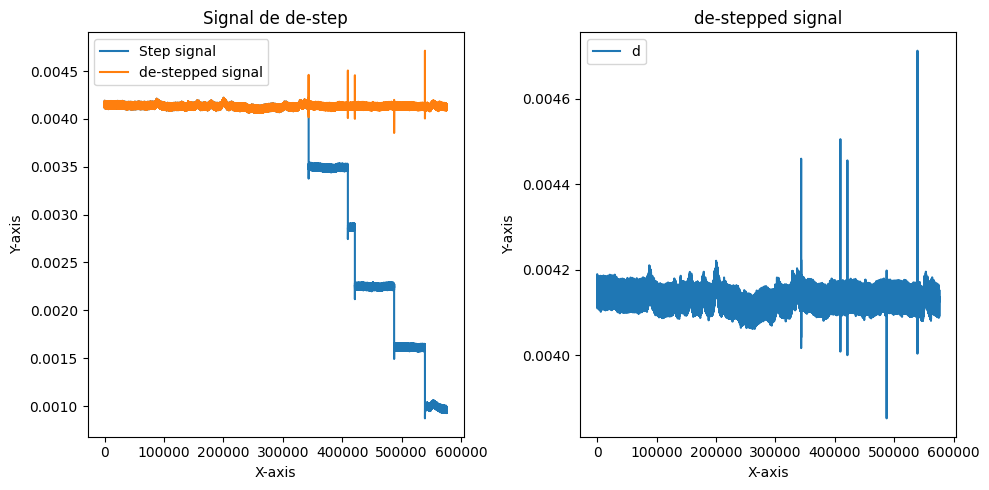
\includegraphics[width=.8\textwidth]{figures/step_removal_real.png}
        \caption{Application of the step removal algorithm.}
        \label{fig:data}
    \end{figure}
\end{frame}

\begin{frame}{Ringing removal}

    Ringing artefacts are caused by the antialiasing filter. First, we estimate the parameters of this filter to model its impulse response and cancel it, which removes ringing artefacts.
    \begin{figure}
        \centering
        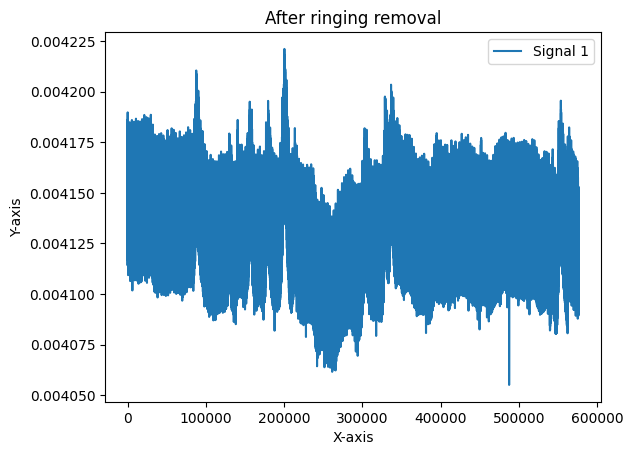
\includegraphics[width=.4\textwidth]{figures/ringing_removal_real.png}
        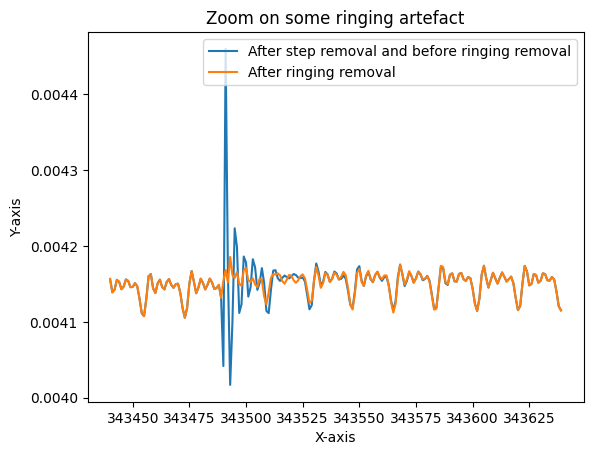
\includegraphics[width=.4\textwidth]{figures/ringin_removal_zoom.png}
        \caption{Left: A full signal. Right: zoom on an artefact}
        \label{fig:data}
    \end{figure}
\end{frame}


\section[\color{white} Application]{Application : Reconstruction}\label{sec:results}

\begin{frame}{Data}
  4 min long MEG recording at 2400Hz with 303 channels\\$\implies 174'528'000$ samples

  We used only 16 channels because we have limited compute capabilities.
\end{frame}

\begin{frame}{A complete pipeline for preprocessing}
    Remove steps \(\to\) Remove ringing artefacts \(\to\) Robust detrend \(\to\) Detect outliers \(\to\) Inpainting \(\to\) Robust rereference.
    \begin{figure}
        \centering
        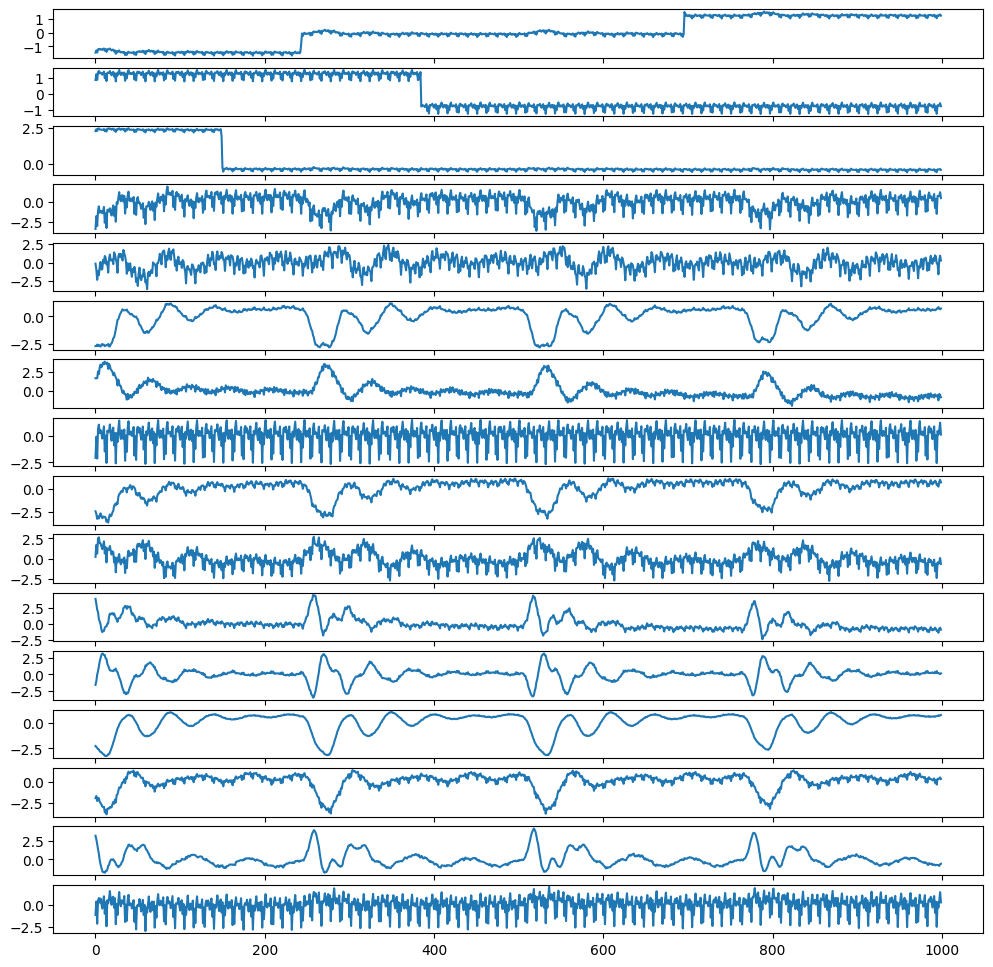
\includegraphics[width=.45\textwidth]{figures/data_raw.png}
        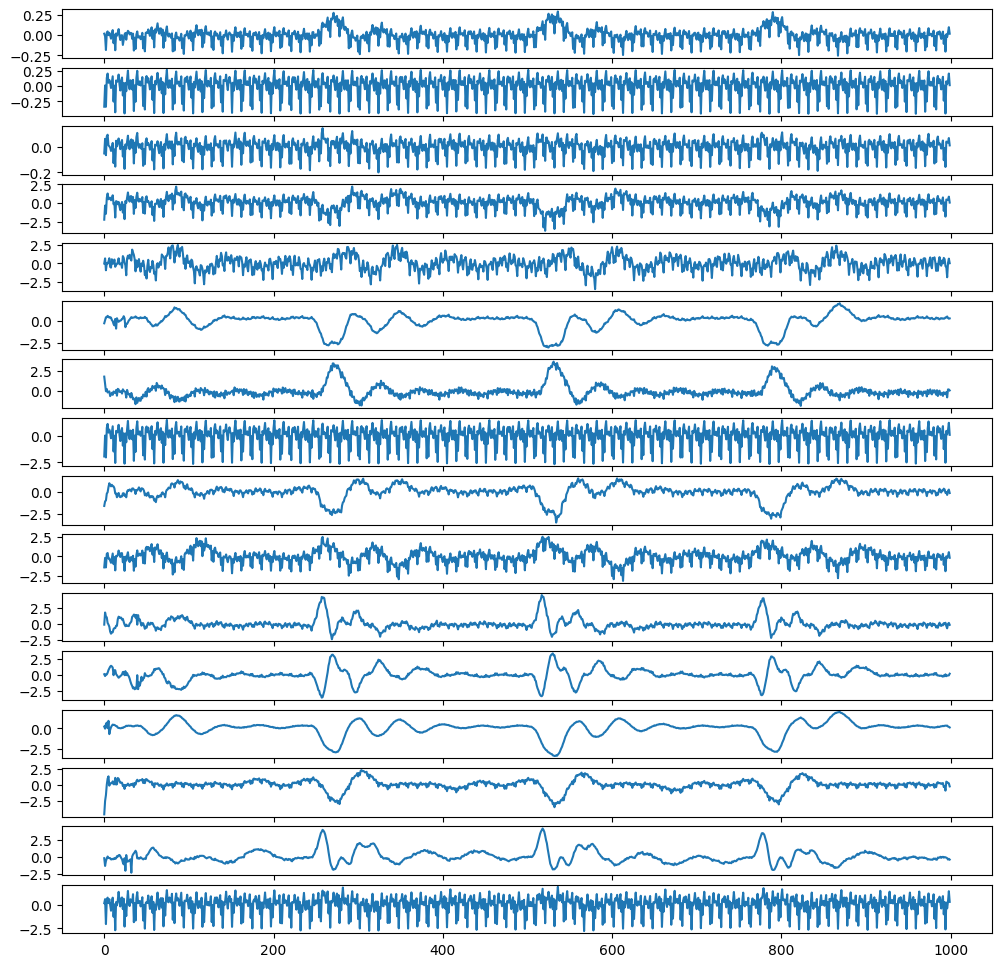
\includegraphics[width=.45\textwidth]{figures/data_clean.png}
        \caption{Left: Raw MEG data. Right: Cleaned MEG data}
        \label{fig:data}
    \end{figure}
\end{frame}

\begin{frame}{Results}
    \begin{figure}
        \centering
        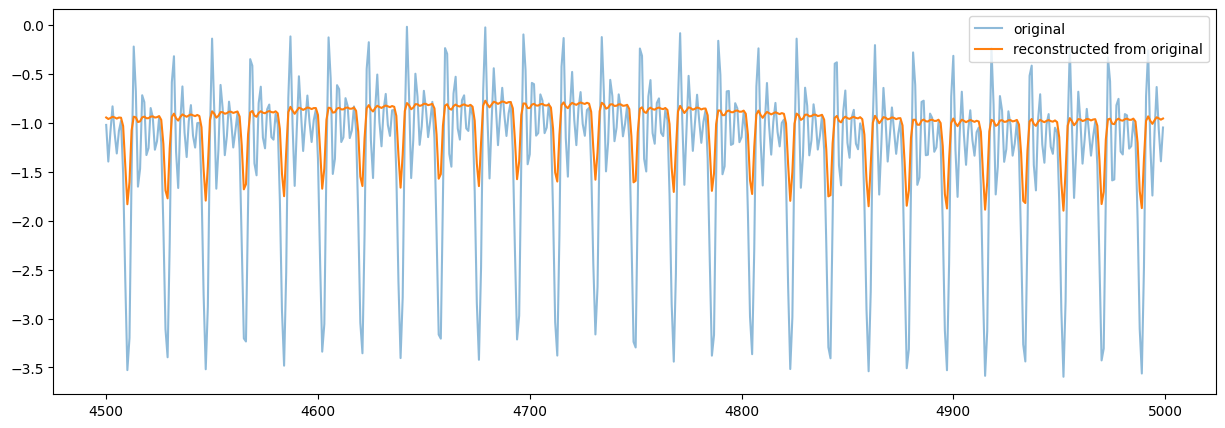
\includegraphics[width=.77\textwidth]{figures/recons}\\
        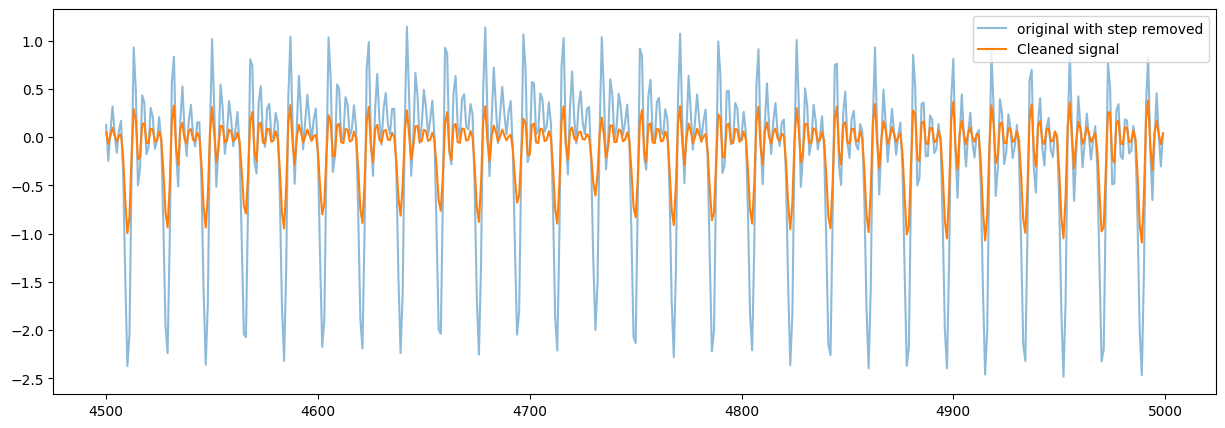
\includegraphics[width=.77\textwidth]{figures/recons_clean}
        \caption{Top: Raw MEG and its reconstruction. Bottom: Cleaned MEG with its reconstruction}
        \label{fig:recons}
    \end{figure}
\end{frame}

\begin{frame}[allowframebreaks]
    \frametitle{References}
    \printbibliography
\end{frame}

\end{document}
